
\section[Examples]{Examples}
\label{sec:example}
\addcontentsline{toc}{section}{\thesection. Examples}


\subsection[EM Control]{EM Control}
\label{sec:emcontrol}
\addcontentsline{toc}{subsection}{\thesubsection. EM Control}

The \pkg{EMCluster} provides a control function \code{.EMControl} and
three default controls \code{.EMC}, \code{.EMC.Rnd}, and \code{.EMC.Rndp}
which are useful to manipulate different initializations.
By default \code{.EMC} is for {\it emEM},
\code{.EMC.Rnd} is for {\it RndEM}, while
\code{.EMC.Rndp} is for {\it RndEM} but with different flavor.

For larger data or high overlaps data,
general users may want to increase the initial iteration
(\code{.EMC$short.iter})
which can improve the clustering results.
However, the initialization also cost computing time and may take longer
to obtain stable initials especially for large number of clusters or
high overlap data.

Anyway, these also provide advanced developers to explore new initialization
methods.
We give two examples next for unsupervised and semi-supervised clusterings
utilizing all initialization methods in \pkg{EMCluster}.


\subsection[Unsupervised Clustering]{Unsupervised Clustering}
\label{sec:unsupervised}
\addcontentsline{toc}{subsection}{\thesubsection. Unsupervised Clustering}

In an \proglang{R} session, you can run the demo as
\begin{Code}[title=unsupervised]
R> demo(allinit, 'EMCluster', ask = F)
\end{Code}
which clusters a small dataset \code{da1} of \pkg{EMCluster} with
$10$ clusters. The data set has only $500$ observations in two dimensions.

This demo provides a plot
with four unsupervised clustering results including
{\it emEM} (em), {\it RndEM} (Rnd), {\it RndEM+} (Rnd+)
and {\it svd} (svd) where colors and symbols
indicate different clusters as in the Figure~\ref{fig:unsupervised}.
The {\it RndEM+} has different settings to the {\it RndEM}.
The demo also compares classifications with true ids using adjusted
Rand index~\citep{Hubert1985} which has value before $0$ (bad results)
and $1$ (perfect match) as in the Table~\ref{tab:unsupervised}.

\begin{figure}[h]
\caption{Unsupervised clustering results for four initializations.}
\centering
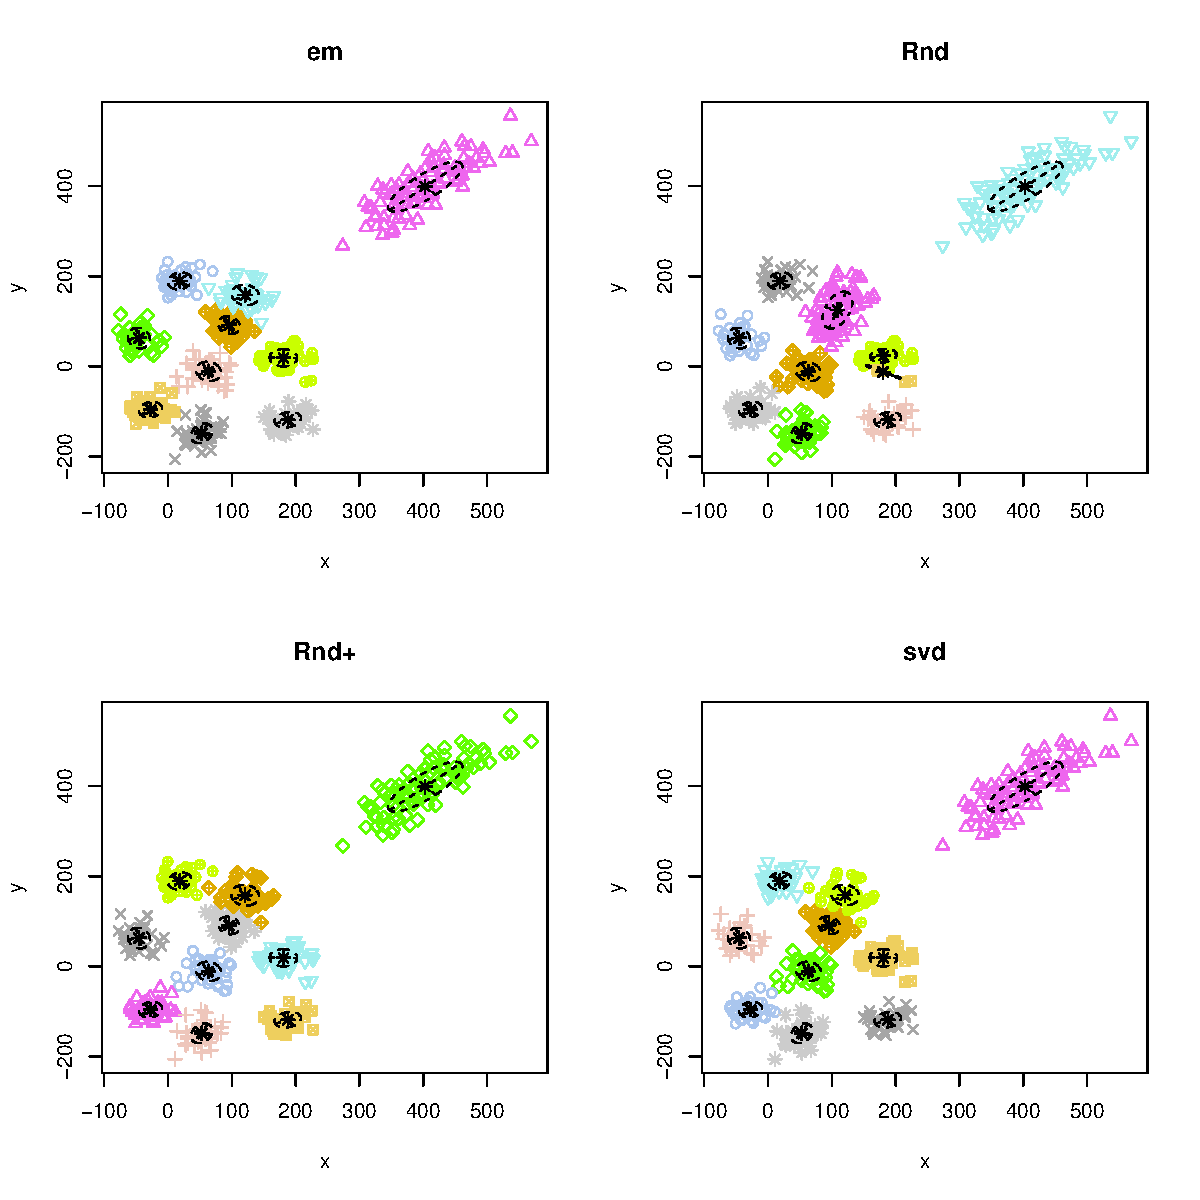
\includegraphics[width=4in]{./EMCluster-include/allinit}
\label{fig:unsupervised}
\end{figure}

\begin{table}[h]
\centering
\begin{tabular}{l|rr} \hline \hline
     &      logL &      adjR \\ \hline
em   & -5657.603 & 0.9929422 \\
Rnd  & -5658.984 & 0.9096019 \\
Rnd+ & -5657.612 & 0.9929422 \\
svd  & -5657.600 & 0.9929422 \\ \hline \hline
\end{tabular}
\caption{Comparison by
log likelihood (logL) and adjusted Rand index (adjR) of four
initializations.}
\label{tab:unsupervised}
\end{table}




\subsection[Semi-supervised Clustering]{Semi-supervised Clustering}
\label{sec:semi-supervised}
\addcontentsline{toc}{subsection}{\thesubsection. Semi-supervised Clustering}

Inside an \proglang{R} session, you can run the demo as
\begin{Code}[title=unsupervised]
R> demo(allinit_ss, 'EMCluster', ask = F)
\end{Code}
which clusters a small dataset \code{da1} in \pkg{EMCluster} with
$10$ clusters.

We randomly choose $6$ clusters, then select $50\%$ of data for
each cluster. There are about $170$ points are labeled with true
which are prior information, then we cluster the rest $330$ points
into $10$ clusters by semi-supervised clustering.

This demo provides a plot
with three semi-supervised clustering results including
{\it emEM} (em), {\it RndEM} (Rnd), {\it RndEM+} (Rnd+) where
colors and symbols
indicate different clusters as in the Figure~\ref{fig:semi-supervised}.
Note that {\it svd} method is not implemented for semi-supervised clustering.
The demo also compares classifications with true ids using adjusted
Rand index as in the Table~\ref{tab:semi-supervised}.

Comparing with the Table~\ref{tab:unsupervised},
the semi-supervised clustering provides better results
than the unsupervised clustering in terms of
higher log likelihood (logL) and adjusted Rand index (adjR).
The reason is that some tiny clusters are not seeded at the initial step in
unsupervised clustering, therefore, a few prior information from there
can substantially improve accuracy by the semi-supervised clustering.


\begin{figure}[h]
\caption{Semi-supervised clustering results for three initializations.}
\centering
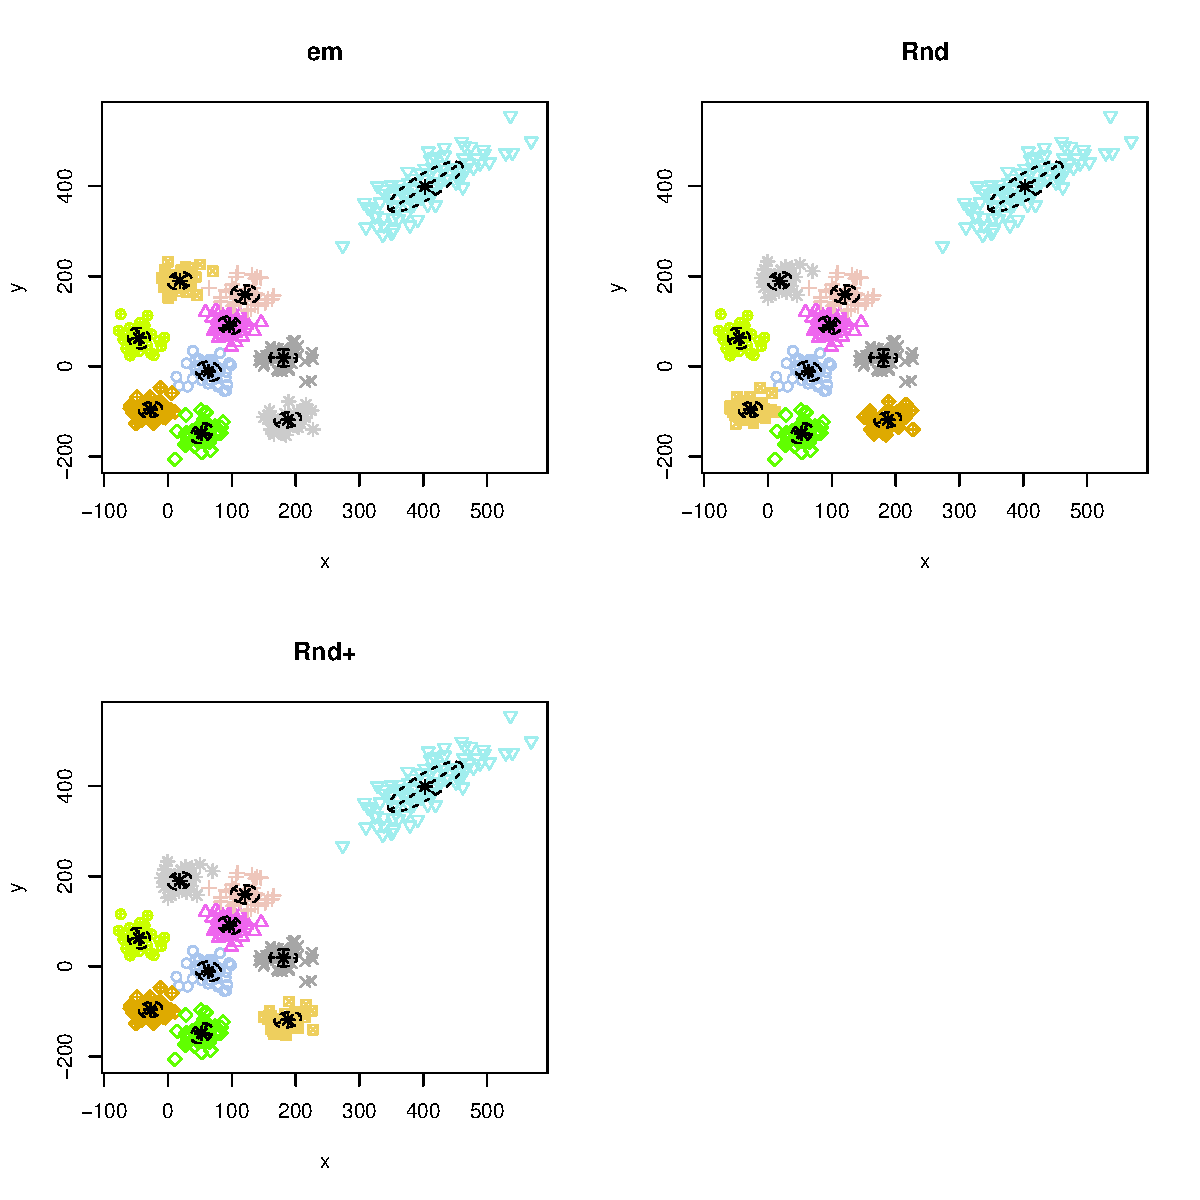
\includegraphics[width=4in]{./EMCluster-include/allinit_ss}
\label{fig:semi-supervised}
\end{figure}

\begin{table}[h]
\centering
\begin{tabular}{l|rr} \hline \hline
     &      logL &      adjR \\ \hline
em   & -5657.882 & 0.9938959 \\
Rnd  & -5657.880 & 0.9938959 \\
Rnd+ & -5657.881 & 0.9938959 \\ \hline \hline
\end{tabular}
\caption{Comparison by
log likelihood (logL) and adjusted Rand index (adjR) of three
initializations.}
\label{tab:semi-supervised}
\end{table}
